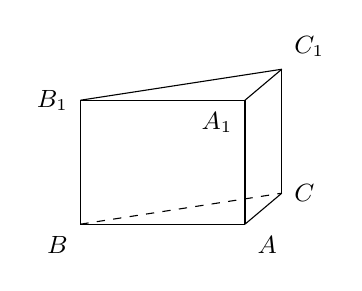
\begin{tikzpicture}[x=0.82cm,y=0.82cm,every node/.style={font=\small}]
  % Source-faithful triangular-prism topology; projection lengths are schematic.
  \coordinate (B)  at (0,0);
  \coordinate (A)  at (2.55,0);
  \coordinate (C)  at (3.12,0.48);
  \coordinate (B1) at (0,1.92);
  \coordinate (A1) at (2.55,1.92);
  \coordinate (C1) at (3.12,2.40);

  % Solid edges shown in the source diagram.
  \draw (B) -- (A);
  \draw (A) -- (C);
  \draw (A) -- (A1);
  \draw (B) -- (B1);
  \draw (C) -- (C1);
  \draw (B1) -- (A1);
  \draw (A1) -- (C1);
  \draw (B1) -- (C1);

  % The hidden base edge BC is dashed in the source.
  \draw[dashed] (B) -- (C);

  \node[below left=1pt] at (B) {$B$};
  \node[below right=1pt] at (A) {$A$};
  \node[right=1pt] at (C) {$C$};
  \node[left=1pt] at (B1) {$B_1$};
  \node[below left=1pt] at (A1) {$A_1$};
  \node[above right=1pt] at (C1) {$C_1$};
\end{tikzpicture}
